\documentclass{report}
\usepackage[utf8]{inputenc}
\usepackage{graphicx}
\usepackage[siunitx ,europeanresistors ,americaninductors]{circuitikz}
\usepackage{tikz}
\usepackage{pgfplots}

\title{P02 Latex}
\author{arif.mammadov }
\date{March 2018}

\begin{document}

\maketitle

\chapter{
Theoretical part
}

\begin{center}
\begin{circuitikz}[scale=1.2, every node/.style={transform shape}] \draw
(0,0) to[battery=$V$] (0,4)
      to[resistor=$R1$] (6,4)
      to[resistor=$R2$] (6,0) -- (0,0)
;
\end{circuitikz}
\end{center}
\begin{center}
\begin{tikzpicture}
\begin{axis}[
    axis lines = left,
    xlabel = $U(R2)$,
    ylabel = {$f(R2)$},
]
%Below the red parabola is defined
\addplot [
    domain=-10:10, 
    samples=100, 
    color=red,
]
{0.24*x};
\addlegendentry{$I * R2$}
\end{axis}
\end{tikzpicture}
\end{center}
\section{
Circuit calculation
}



\begin{tabular}{ |c|c| } 
 \hline
 R1 & 2 \\ 
 R2 & 3 \\ 
 V1 & 1.2 \\ \
 U_R_1 & 0.48 \\ 
 U_R_2 & 0.72 \\ 
 \hline
\end{tabular}

\chapter{Practical part}

\section{Work with GEDA programs}

\subsection{Work with gschem\cite{program1}}
\text{In this section we opened Gschem program with help of command "gschem". Then we created the circuit based on digits on our ID}

\subsection{Work with gnetlist}

\subsection{Work with ngspice\cite{program2}}
\text{With the help of ngspice we declared time to see our values in a graphical form. Then we got our graphs by the function "plot".}

\begin{center}
    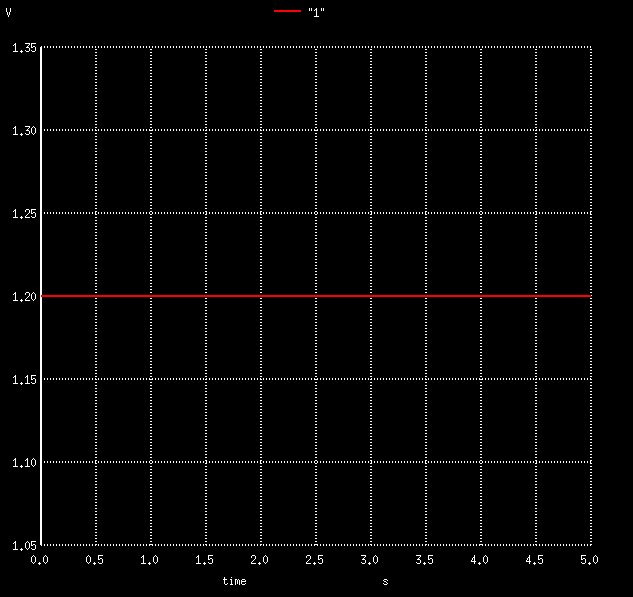
\includegraphics[scale=0.4]{1.png}
    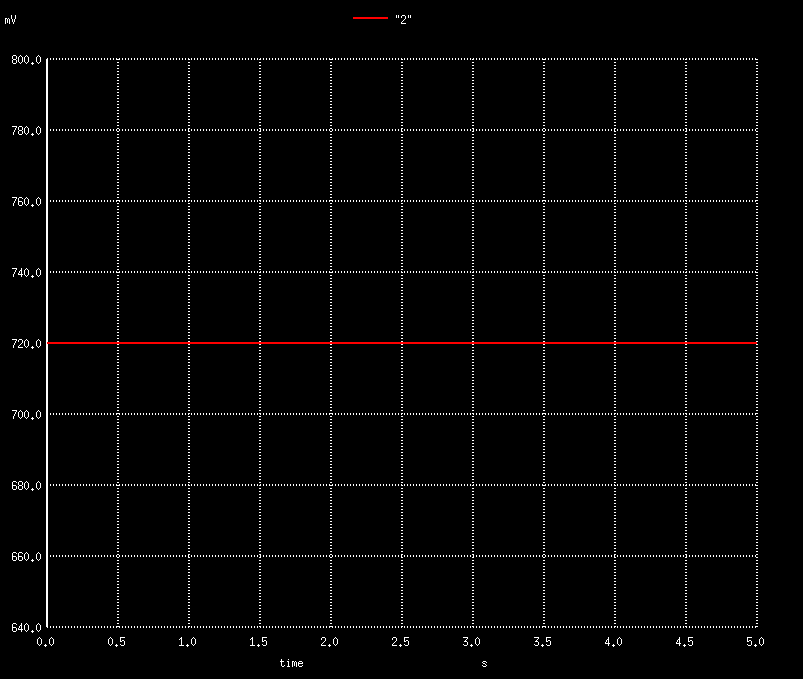
\includegraphics[scale=0.4]{2.png}
\end{center}

\section{work with QUCS programs}
\text{Since it was optional to do this part, I have skipped this section.}


\begin{thebibliography}{9}
\bibitem{program1}
The program for drawing circuits
\bibitem{program2}
The program for plotting functions and circuits
\end{thebibliography}
\end{document}
